\item Problem 31.3-1

\begin{align*}
    & B = 2000 \\
    & N_N = 1.85 \\
    \intertext{Constant overflow}
    L_N &= \frac{B}{N_N} \\
    L_N &= \frac{2000}{1.85} = 1081 \\
    & A_N = 120 \\
    C_N &= L_N - A_N \\
    C_N &= 1081 - 120 = 961 \\
    \intertext{Liquid phase of slurry outlet}
    y_{A,N} &= \frac{120}{1081} \\
    \Aboxed{y_{A,N} &= 0.111} \\
    \intertext{Mass balance on A}
    A_0 + A_{N+1} &= A_N + A_1 \\
    800 + 20 &= 120 + A_1 \\
    A_1 &= 700 \\
    \intertext{Mass balance on C}
    C_0 + C_{N+1} &= C_N + C_1 \\
    50 + 1310 &= 961 + C_1 \\
    C_1 &= 398 \\
    \intertext{Solvent outlet}
    x_{A,1} &= \frac{A_1}{A_1 + C_1} \\
    x_{A,1} &= \frac{700}{700 + 398} \\
    \Aboxed{x_{A,1} &= 0.637}
\end{align*}

\begin{align*}
    \intertext{Stage analysis:}
    x_{A\Delta} &= \frac{L_0 y_{A,0} - V_1 x_{A,1}}{L_0 - V_1} \\
    x_{A\Delta} &= \frac{850 \cdot 0.941 - 1098 \cdot 0.637}{850 - 1098} \\
    x_{A\Delta} &= -0.401 \\
    N_\Delta &= \frac{B}{L_0 - V_1} \\
    N_\Delta &= \frac{2000}{850 - 1098} \\
    N_\Delta &= -8.03 \\
\end{align*}

The operating line is constant at $N=1.85$. Plot operating line, start and end points, and $\Delta$ point and step off stages graphically.

\begin{align*}
    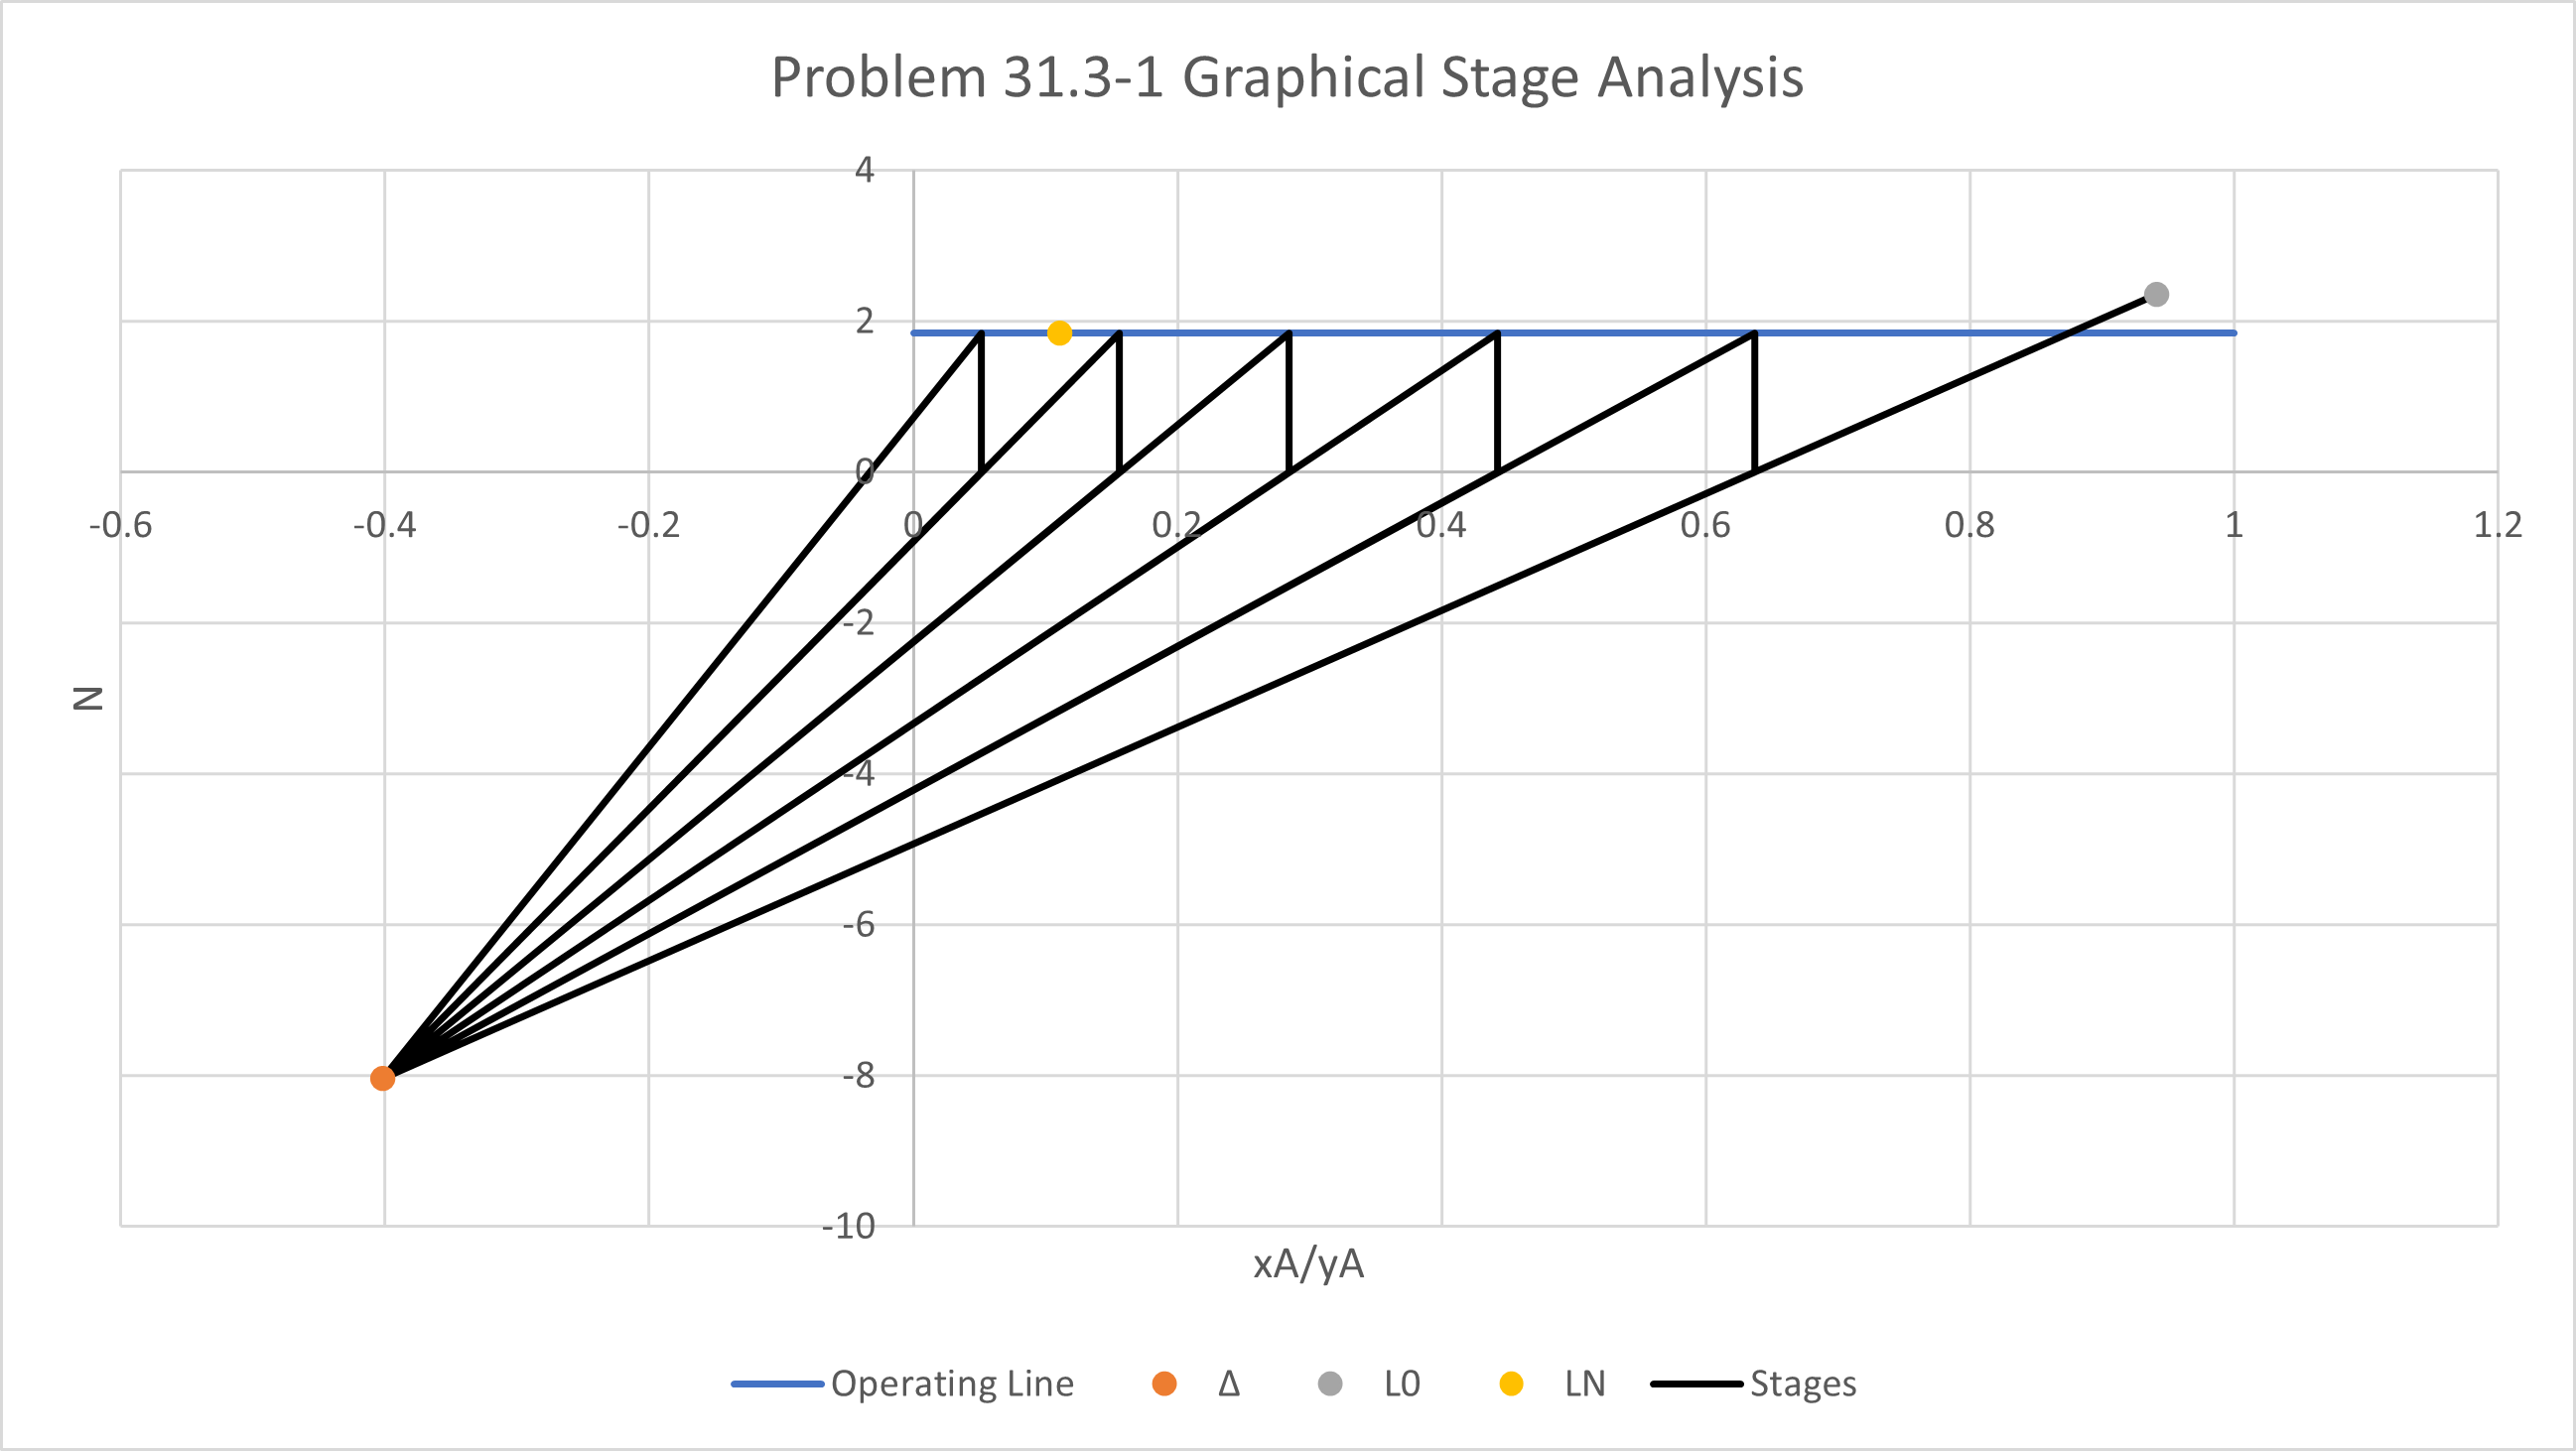
\includegraphics[width=0.8\textwidth]{assets/p5.png}
\end{align*}

Start point falls between stage 4 and 5. $\boxed{N \approx 4.4}$